% USER MANUAL FOR SPOTMACHINE
%
% To compile, simply run:
% $ pdflatex usermanual.tex
%
% Nice overview of most basic LaTeX commands:
% http://en.wikibooks.org/wiki/LaTeX/Document_Structure

\documentclass[a4paper,12pt]{report}
\usepackage{url,graphicx}
\begin{document}
\title{SpotMachine \\ Usermanual}
\author{Thomas Pryds}
\date{June 2013}

\maketitle

\tableofcontents

\chapter{Introduction}

SpotMachine lets you record and sequentially play pieces of audio. It is intended for commercial audio spots running in shopping malls, supermarkets, amusement parks, and other places with the need of reaching out to masses through repetitive audio clips.

\section{Features}
\begin{itemize}
\item Arrange spots for rotation
\item Play spots by interval (specify pause time)
\item Play spots by schedule (specify point in time)
\item Record your own audio spots
\item Easy and simple user interface
\item Keep spots for later use
\item Have the same spot multiple times in the same rotation
\item No limit on number of spots
\item Audio normalization for uniform spot messages
\item Available in English and Danish (and easily extended into more languages)
%\item Upcoming: Import spot from audio file
\end{itemize}

\section{Licensing}
SpotMachine is released under the GPL license which means that you are allowed to use it for whatever reason you want, be it commercial or non-commercial. You can even download the source code and change the behaviour of the program if you so desire.

You are also allowed to redistribute SpotMachine, with or without changes, as long as you do so under the same license, and provide the source code for whichever changes you have made. You can read the full details of the licence in the LICENSE text file which is distributed with SpotMachine.

\chapter{Installation}
SpotMachine runs on all major operating systems, and its only requirement is a working, current install of Java. If you do not have Java on your system, you should download and install it from \url{http://java.oracle.com} or through your operating system's package management system, prior to installing SpotMachine.

\section{Windows}
An easy-to-use installer package is available for Windows. Just download it from the SpotMachine website, run it, and follow the instructions on-screen. The installer, of course, provides easy, Windows-integrated means of uninstalling SpotMachine.

\section{Ubuntu and Debian}
On systems that use the Debian packaging system, you can make use of the precompiled deb package which is provided through the SpotMachine website. After downloading the file, just install it by either double clicking it, or by the following command: \texttt{sudo dpkg -i spotmachine-X.X.deb}. This package assumes you have installed Java through the package system; if not, it will try to install it for you.

\section{Other Linux, Mac, and Others}
Currently, no installer is provided for these systems, unfortunately. However, installation is not very complicated: Download the pre-compiled package spotmachine*.bin.tar.bz2 (where * is the newest version number), uncompress it to somewhere on your harddrive, and follow the instructions in the INSTALL text file.

\section{Sources}
If you wish to compile SpotMachine yourself, you can download the source code package from the SpotMachine website. Uncompress the file to somewhere on your harddrive, and follow the instructions in the INSTALL text file.

\chapter{Daily Usage}
All features of SpotMachine are, directly or indirectly, available from the main window. This is where you can see an overview of recorded spots, which spots are currently in rotation, when they are playing.

\begin{figure}[h]
\centering 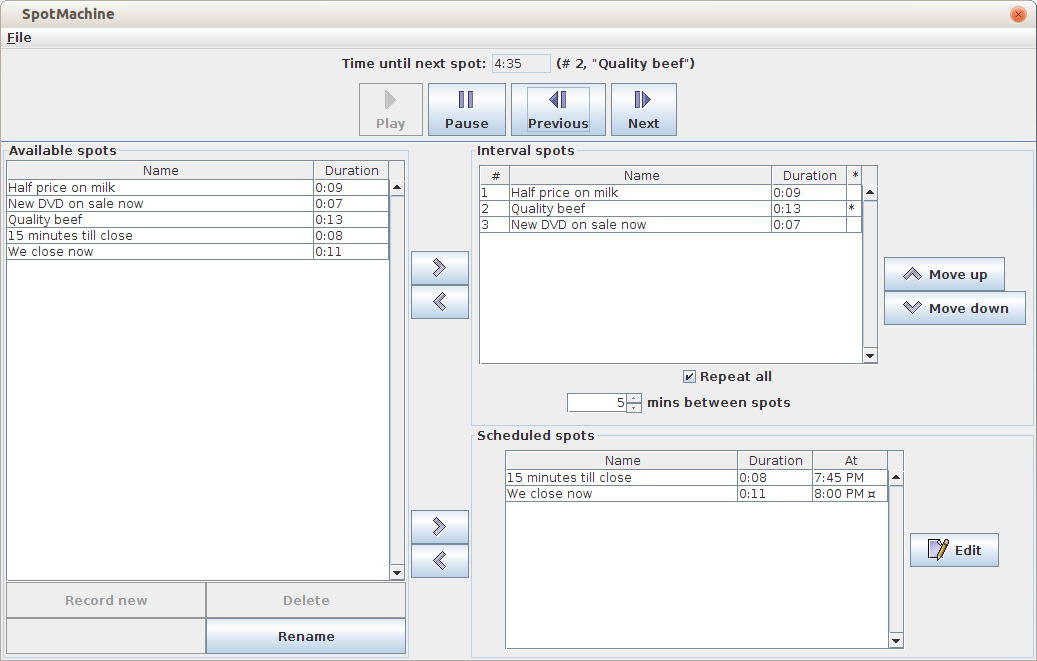
\includegraphics[width=130mm]{mainwindow.png}
\caption{Main window.}
\end{figure}

The main window is split up in three parts:
\begin{itemize}
\item The top part containing the {\bf control buttons} Play, Pause, Previous and Next.
\item The left side containing all {\bf available spots}.
\item The right side containing spots currently in {\bf interval rotation} and spots currently in {\bf scheduled rotation}.
\end{itemize}

\section{Control Buttons}
At the top you control whether the current rotation spots are to be played, or if they're on pause. For normal use, the SpotMachine would typically be set to ``Play'' and then left alone. Pause would typically be used while recording new spots -- in fact you cannot record new spots, unless pause in on. Note that pausing only affects spots that are on interval rotation (see further down for an explanation), not those set for scheduled play. %This behaviour might change in a future version of SpotMachine.

\section{Available Spots}
The left side of the main window shows a list of recorded spots. These spots are not necessarily set up for interval or scheduled play (more about this later) -- this is a list of all spots available to you at any given moment. By selecting a spot in this list, you may rename it, delete it, or set it up for interval or scheduled play.

\subsection{Recording a New Spot}
You can record a new spot through a connected microphone. All new spots will show up in the Available spots list. To do so, click the Record new button below the Available spots list, and a new window will pop up, from which you can control the recording itself.

\begin{figure}[h]
\centering 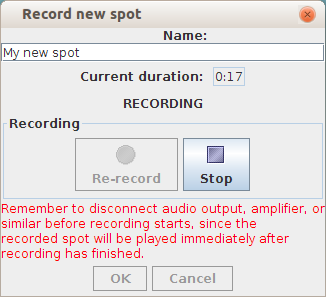
\includegraphics[width=50mm]{recorddialogue.png}
\caption{Record new spot window.}
\end{figure}

Here, you can give the spot a name, which will appear in spot lists. Be sure to give the spot a descriptive name, and note that you {\em are} able to give the exact same name to two different spots! You are able to type in a name either before, during or after recording a spot.

In the middle of the window are two buttons. The left button will start the actual recording of the spot. The right one will stop recording. While recording, you can keep track of the length of the spot just above the record and stop buttons. Here, you can also see, whether SpotMachine is currently recording, or not.

When you click the Stop button, the recording is immediately played back once, to let you hear if everything is like you want it to be. For this reason, be sure to check that you are not connected to an amplifier or in some other way publicly transmitting before starting to record new spots. Connecting a set of headphones instead is recommended. If the recording does not sound ok, you can click the record button again, which discards the previous recording and starts a new one.

If you like what you hear, click the OK button, and the new spot is added to the Available spots list in the main window. If instead, you click the Cancel button, any newly recorded spot is discarded, and the recording window is closed.

\subsection{Deleting a Spot}

\begin{figure}[h]
\centering 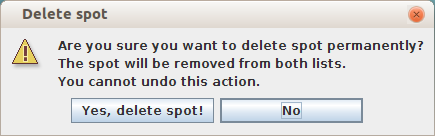
\includegraphics[width=60mm]{deletespotdialogue.png}
\caption{Delete spot window.}
\end{figure}

If you decide you will not need a certain spot ever again, you can delete it entirely from disk. You do so by selecting the spot in the Available spots list and click the Delete button. You will be met with a brief acknowledge window, just to make sure that you are not deleting something by accident. If you delete a spot that is currently also in the Interval spots and/or Scheduled spots lists, the spot will also be removed from these lists.

Note, this function deletes the spot's audio file from disk, so it is non-reversible. If you are probably going to use a spot at some later point, but not now, you can just let it sit in the Available spots list for later use.

\subsection{Renaming a Spot}
Changing the name of a spot after it has been recorded is possible through the Rename button. By clicking it you will be presented with a small popup window that allows you to do so. Bear in mind, that spots are not recognized by the program from their names, so it is perfectly possible to name two spots exactly the same, for whatever reason you might have to do so. In most cases, this is discouraged, though, as to not confuse spots with each other.

\section{Interval and Scheduled Spots}
The right side of the main window is, in turn, divided into two lists of spots. The spots shown in these two lists have the fact in common that they are set up for being played in one way or another; playlists, if you like. Note, that a spot can easily appear in both lists -- in fact, it can appear more than once in either list.

{\em Interval spots}: The first one is a list of spots that are played sequentially with a given interval between them, e.g. five minutes. In a commercial setting like a supermarket, this would be used for promoting special offers (``Half price on milk today''), service announcements (``Extended opening hours tomorrow''), etc.

{\em Scheduled spots}: The second list contains spots which are played at a given point in time, e.g. at 7:45~PM every Monday to Friday. This might be used for time based service announcements (like in our supermarket example: ``15 minutes till closing time'', etc.).

\subsection{Adding a Spot as an Interval Spot}
Between the Available spots list and the Interval spots list, you see two arrow buttons. The arrow point to the right copies a spot into the Interval spots list. You can copy the same spot into the list several times, if you have a certain spot that you want to play more often than the others.

\subsection{Changing the Properties of Interval Spots}
The play order is given in the list, and by selecting a spot and clicking the Move up and Move down buttons, you can change this to your linking.

Below the list you can choose whether to start over when the end of the list is reached (by checking the Repeat all checkbox). Also, you can set the amount of minutes between playing each spot.

\subsection{Adding a Spot as a Scheduled Spot}

\subsection{Changing the Properties of Scheduled Spots}
%editing an existing scheduled spot

\end{document}

